\documentclass{article}

\usepackage{xcolor}
\usepackage{listings}
\usepackage{textcomp}
\usepackage{ulem}
\usepackage{listings}
\usepackage[T1]{fontenc}
\usepackage{fancyhdr} % Required for custom headers
\usepackage{lastpage} % Required to determine the last page for the footer
\usepackage{extramarks} % Required for headers and footers
\usepackage{graphicx} % Required to insert images
\usepackage{courier} % Required for the courier font

% Margins
\topmargin=-0.45in
\evensidemargin=0in
\oddsidemargin=0in
\textwidth=6.5in
\textheight=9.0in
\headsep=0.25in

\linespread{1.1} % Line spacing

% Set up the header and footer
\pagestyle{fancy}
\lhead{} % Top left header
\rhead{\firstxmark} % Top right header
\lfoot{\lastxmark} % Bottom left footer
\cfoot{} % Bottom center footer
\rfoot{Page\ \thepage\ of\ \protect\pageref{LastPage}} % Bottom right footer
\renewcommand\headrulewidth{0.4pt} % Size of the header rule
\renewcommand\footrulewidth{0.4pt} % Size of the footer rule

\setlength\parindent{0pt} % Removes all indentation from paragraphs

\lstset{
    inputencoding=utf8,
    tabsize=4,
    rulecolor=,
    numbers=left,
    upquote=true,
    columns=fixed,
    showstringspaces=false,
    extendedchars=true,
    breaklines=true,
    prebreak=\raisebox{0ex}[0ex][0ex]{\ensuremath{\hookleftarrow}},
    frame=single,
    showtabs=false,
    showspaces=false,
    showstringspaces=false,
    basicstyle=\small\ttfamily,
    identifierstyle=\ttfamily,
    keywordstyle=[1]\ttfamily\color{blue},
    keywordstyle=[2]\ttfamily\color{purple},
    keywordstyle=[3]\ttfamily\colorbox{yellow},
    commentstyle=\ttfamily\color[rgb]{0.133,0.545,0.133},
    stringstyle=\ttfamily\color[rgb]{0.627,0.126,0.941},
}

\makeatletter
\lstdefinelanguage{llvm}{
  morecomment = [l]{;},
  morestring=[b]", 
  sensitive = true,
  morekeywords=[1]{
    define, declare, global, constant,
    internal, external, private,
    linkonce, linkonce_odr, weak, weak_odr, appending,
    common, extern_weak,
    thread_local, dllimport, dllexport,
    hidden, protected, default,
    except, deplibs,
    volatile, fastcc, coldcc, cc, ccc,
    x86_stdcallcc, x86_fastcallcc,
    ptx_kernel, ptx_device,
    signext, zeroext, inreg, sret, nounwind, noreturn,
    nocapture, byval, nest, readnone, readonly, noalias, uwtable,
    inlinehint, noinline, alwaysinline, optsize, ssp, sspreq,
    noredzone, noimplicitfloat, naked, alignstack,
    module, asm, align, tail, to,
    addrspace, section, alias, sideeffect, c, gc,
    target, datalayout, triple,
    blockaddress
  },
  morekeywords=[2]{
    add, fadd, sub, fsub, mul, fmul,
    sdiv, udiv, fdiv, srem, urem, frem,
    and, or, xor,
    icmp, fcmp,
    eq, ne, ugt, uge, ult, ule, sgt, sge, slt, sle,
    oeq, ogt, oge, olt, ole, one, ord, ueq, ugt, uge,
    ult, ule, une, uno,
    nuw, nsw, exact, inbounds,
    phi, call, select, shl, lshr, ashr, va_arg,
    trunc, zext, sext,
    fptrunc, fpext, fptoui, fptosi, uitofp, sitofp,
    ptrtoint, inttoptr, bitcast,
    ret, br, indirectbr, switch, invoke, unwind, unreachable,
    malloc, alloca, free, load, store, getelementptr,
    extractelement, insertelement, shufflevector,
    extractvalue, insertvalue,
  },
  alsoletter={\%},
  keywordsprefix={\%},
}
\makeatother

\title{
\vspace{2in}
\textmd{\textbf{Precise GC Support in LLVM}}\\
\vspace{0.1in}\large{COMS\ W4115}\\
\vspace{0.1in}\large{\textit{Alfred A. Aho}}
\vspace{2in}
}
\author{Ramkumar Ramachandra, rr2893}
\begin{document}
\maketitle
\newpage
\tableofcontents
\newpage
\section{A brief introduction to LLVM}
LLVM, which originally stood for Low Level Virtual Machine, is a 2003
project led by Chris Lattner. Today, it is an indispensable piece of
compiler infrastructure which both compiler writers and users must be
familiar with. It contains C, C++ and Objective-C compilers, sharing a
common backend infrastructure. It is currently being used in many
C-like language projects like OpenCL and Rust.\\

LLVM has a common IR, or intermediate representation, that different
frontends must target; the backend works on optimizing this IR via a
series of optimization passes and emits target-specific bytecode.

It looks something like C:
\begin{lstlisting}[language=llvm]
define %value_t* @0() {
entry:
  %value = call i8* @malloc(i64 ptrtoint (%value_t* getelementptr (%value_t* null, i32 1) to i64))
  %malloc_value = bitcast i8* %value to %value_t*
\end{lstlisting}

\begin{lstlisting}[language=llvm]
  switch i32 %load19, label %default [
    i32 1, label %caseN
    i32 4, label %caseN24
  ]

default:                               ; preds = %entry
  %load21 = load i1* %boxptr10
  br label %switchcont

caseN:                                 ; preds = %entry
  %boxptr22 = getelementptr inbounds %value_t* %malloc_value8, i32 0, i32 1
  %load23 = load i64* %boxptr22
  %intbool = icmp eq i64 %load23, 0
  %. = select i1 %intbool, i1 false, i1 true
  br label %switchcont
\end{lstlisting}
With a minimal set of well-defined instructions, the optimizer has a
relatively easy time operating.\\

The important thing to note about control flow is that the IR is an
SSA. Single Static Assignment means that each variable is defined
before it is used, and is assigned exactly once. A phi instruction is
required to unify values from different basic blocks:
\begin{center}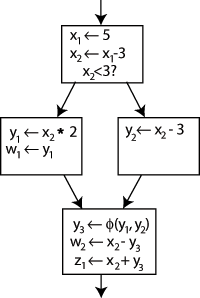
\includegraphics[scale=0.8]{ssa}\end{center}

\section{The need for garbage collection}
A garbage collector gives the program a view of infinite memory, and
frees it up from making memory management decisions. Consider the
program:
\begin{lstlisting}[language=c]
int main() {
	int *v = malloc(3 * sizeof(int));
	...
	v++; // We permanently lose a handle on v[0];
	...
	free(v); // 1 int leaked!
}
\end{lstlisting}
$v$ is a stack-allocated variable which points to memory for 3
integers on the heap. The program happens to lose reference to one of
those integers; hence, a subsequent free would result in a leak. One
might argue that only C allows such semantics, but that is not at all
true. Consider:
\begin{lstlisting}[language=ruby]
class IndexPage < Page
  def initialize(filename)
    if filename.contains('.index')
      @permalink = filename.split('.index')[0]
    end
    @target = "#{@permalink}.html"
  end
end
\end{lstlisting}
Here, the semantics of a hypothetical free are very complicated. What
happens when filename.split('.index') returns N splits? Only the first
split is captured in a variable, so what happens to the other N-1
splits? Does the first split share memory with ``filename''? Is it
safe to free ``filename'' at the end of the function? As Ruby
designers refine the language constantly, and optimize things, must
they always worry about the lifetimes and reference counts of
variables?\\

To illustrate how reference counting works, let's implement a
simplistic version of shared pointers in C++:
\begin{lstlisting}[language=c++]
template <class T>

class SharedPtr{
public:
	SharedPtr(){
		nRefCount=new int;
		(*nRefCount)=1;
		data=0;
	}
	SharedPtr(T* SpArgument){
		nRefCount=new int;
		this->data=SpArgument;
		(*nRefCount)=1;
	}
	SharedPtr(const SharedPtr &SpArgument){
		this->data = SpArgument.data;
		this->nRefCount = SpArgument.nRefCount;
		(*nRefCount)++;
	}
	SharedPtr& operator=(const SharedPtr &SpArgument){
		// Emulate dtor call, destroy this
		(*nRefCount)--;
		if((*nRefCount)==0){
			delete nRefCount;
			delete data;
		}

		this->data = SpArgument.data;
		this->nRefCount = SpArgument.nRefCount;
		(*nRefCount)++;
		return *this;
	}
	T* get() const{
		return data;
	}
	T& operator*() const{
		return *data;
	}
	T* operator->() const{
		return data;
	}
	~SharedPtr(){
		(*nRefCount)--;
		if((*nRefCount)==0){
			delete nRefCount;
			delete data;
		}
	}
private:
	T* data;
	int* nRefCount;
};
\end{lstlisting}
As you can imagine, it's horribly inefficient. Everytime, there is a
pointer creation, deletion, or assignment, there's the extra
reference-counting overhead.\\

Now, think about what would happen if we wanted to allocate small
segments of memory over and over again:
\begin{lstlisting}[language=c]
int main() {
	int *v[100];
	for (int i = 0; i < 100; i++) {
		v[i] = malloc(sizeof(int));
		...
	}
}
\end{lstlisting}
We need a manager to $mmap$ a slab of memory and hand that bits of it
at each ``malloc'' callsite. As you can imagine, most languages like
Python and Ruby use a slab allocator, instead of calling out to
``malloc'' each time an object is created.\\

The same argument applies to many disparate $free$ calls. Freeing
memory is an expensive operation, and a dedicated routine to batch up
these calls and fire them off when the program is waiting on IO or
something.\\

Hence, we get a garbage collector.

\section{A garbage collection primer}
So the problem statement is quite simple. You have references to the
heap with no corresponding references on the stack. To find the chunks
of memory to free, we obviously have to manage the heap using a custom
allocator. This is the first component of a garbage collector.
\begin{lstlisting}[language=c]
static struct value_t *gcroot;

void *gc_malloc(size_t nbytes) {
	if (nbytes != sizeof(struct value_t))
		return malloc(nbytes);
	struct value_t *v = malloc(nbytes);
	v->gc_marked = 0;
	v->gc_next = gcroot;
	gcroot = v->gc_next;
	return v;
}
\end{lstlisting}
The core component is some kind of marking and sweeping
algorithm. Reachable objects on the heap must be marked via the roots
as reachable. Let's write simplistic mark and sweep routines of a
mark-and-sweep collector:
\begin{lstlisting}[language=c]
void gc_mark(struct value_t *v) {
	v->gc_marked = 1;
	if (v->type_tag == 4)
		for (int i = 0; i < v->array_len; i++)
			v->array_val[i]->gc_marked = 1;
}

void gc_sweep() {
	struct value_t *this = gcroot;

	while (this) {
		if (!(this->gc_marked)) {
			struct value_t *unreachable = this;
			this = unreachable->gc_next;
			free(unreachable);
		} else {
			this->gc_marked = 0;
			this = this->gc_next;
		}
	}
}
\end{lstlisting}

\section{Garbage collection in LLVM, today}
Foom

\section{A taste of practical work required on the road}
The $ExecutionEngine$ changed in this major update of LLVM. Earlier,
users could use $ExecutionEngine.run\_function$ and pass any OCaml
function to it, and use $GenericValue.as\_pointer$ to capture the
return value. Ofcourse, to interpret the return value, they had to go
down to C and use the OCaml-C bindings to extract the value:
\begin{lstlisting}[language=caml]
let result = ExecutionEngine.run_function f [||] ee in
unbox_value (GenericValue.as_pointer result)
\end{lstlisting}
\begin{lstlisting}[language=c]
value mlbox_value(int atype, struct value_t *v) {
	value int_block = caml_alloc(1, 0);
	value bool_block = caml_alloc(1, 1);
	value string_block = caml_alloc(1, 2);
	value array_block = caml_alloc(1, 3);
	value array_value = 0;
	int i;
	if (atype == 3)
		array_value = caml_alloc(v->array_len, 0);
	switch(atype) {
	case 0:
		Store_field(int_block, 0, Val_long(v->int_val));
		return int_block;
	case 1:
		Store_field(bool_block, 0, Val_int(!!v->bool_val));
		return bool_block;
	case 2:
		Store_field(string_block, 0, caml_copy_string(v->string_val));
		return string_block;
	case 3:
		for (i = 0; i < v->array_len; i++) {
			struct value_t *el = (v->array_val)[i];
			value v = mlbox_value(v_to_atype(el), el);
			Store_field(array_value, i, v);
		}
		Store_field(array_block, 0, array_value);
		return array_block;
	...
	}
}
\end{lstlisting}
In 3.5, ExecutionEngine dropped the idea of $GenericValue$, and moved
to using libffi instead. OCaml bindings had to be updated to expose
$get\_pointer\_to\_global$.\\

Then, Rhine had to be updated to use ocaml-ctypes to specify the
structure of the working data:
\begin{lstlisting}[language=caml]
type cvalue_t
let cvalue_t : cvalue_t structure typ = structure "cvalue_t"
let lang_type = field cvalue_t "lang_type" int32_t
let lang_int = field cvalue_t "lang_int" int64_t
let lang_bool = field cvalue_t "lang_bool" char
let lang_string = field cvalue_t "lang_string" (ptr char)
let lang_array = field cvalue_t "lang_array" (ptr (ptr cvalue_t))
let arraysz = field cvalue_t "arraysz" int64_t
let lang_double = field cvalue_t "lang_double" double
let functionptr = field cvalue_t "functionptr" double
let lang_char = field cvalue_t "lang_char" char
let () = seal cvalue_t

let unbox_value value =
  let t = Int32.to_int (getf value lang_type) in
  match t with
    1 -> LangInt (Int64.to_int (getf value lang_int))
  | 2 -> LangBool (bool_of_int (Char.code (getf value lang_bool)))
  | _ -> raise (Error ("Invalid type"))

let run_f f =
  dump_value f;
  let mainty = Foreign.funptr (void @-> returning (ptr cvalue_t)) in
  let mainf = get_pointer_to_global f mainty ee in
  unbox_value (!@ (mainf ()))
\end{lstlisting}
\end{document}